\section{Desarrollo de la solución}

\subsection{Solución Propuesta}

El algoritmo propuesto tiene como propósito la identificación de los componentes moleculares que forman parte de diferentes objetos astronómicos a simular. Para esto, se analizan las líneas  espectrales a partir de los espectros de dichos objetos astronómicos, con el fin de encontrar patrones y predecir su composición.

Para un objeto astronómico, observar sus líneas espectrales puede ayudar a identificar las moleculas que lo componen, dado que para cada estado energético de dichas moléculas, al estar estas presentes en el objeto, se manifiestan en líneas de emisión a lo largo de sus espectros observados en determinadas frecuencias.

El algoritmo toma ventaja de este comportamiento y busca patrones según la presencia de ciertas líneas. Cuando una molecula está presente en la composición de un objeto, probablemente deberían observarse una serie de líneas a lo largo del espectro. Esto significa quee a menor cantidad líneas teóricas observadas de dicha molécula, menor será la probabilidad de que la molécula forme parte de la composición del objeto.

Así, si existe confusión a la hora de identificar una línea espectroscópica entre dos moléculas, es posible realizar una predicción probabilista de la molécula a la cual corresponde dicha línea basándose en la presencia de cada línea teórica a lo largo del espectro que se está observando.


\subsection{Diseño del Prototipo}

Como se mencionó anteriormente, para el diseño del prototipo se utilizó el proyecto ASYDO. La temperatura en estas simulaciones no posee unidades, ya que las magnitudes de las líneas son relativas a la línea más alta de CO, a la cual se le ha asignado un valor arbitrariamente. Esto significa que los valores en sí mismos no poseen un significado.

El proceso para simular los cubos de prueba consistió en encontrar todas las moléculas y todos sus isotopos dentro de un rango de frecuencia. El rango de frecuencia utilizado para estas pruebas fue desde los 602000 MHz hasta los 606000 GHz, aproximadamente, que corresponde a la banda 9 de ALMA. Se corrió un script de líneas combinadas de varios subconjuntos aleatorios de isotopos, subconjunto de tamaño variable del total de moléculas teóricamente existentes en esta ventana de frecuencias utilizada.

El objetivo del algoritmo es entonces recuperar la lista de moléculas con la cual se generaron los cubos de datos. Para realizar esta tarea solo se pueden utilizar los espectrogramas observados. A través de métodos estadísticos se pretende predecir la presencia de ciertas moléculas y validar dichas predicciones al conocerse las moléculas utilizadas para generar las simulaciones.


\begin{figure}[H]
	\begin{center}
		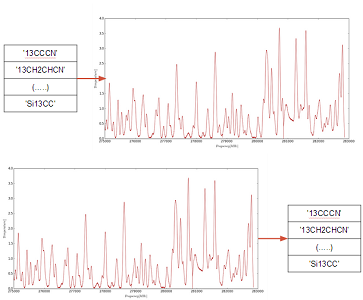
\includegraphics{images/fig0}
		\caption{Se desea recuperar la lista de moléculas con la que se simuló el espectrograma. }
	\end{center}
\end{figure}



\subsection{Implementación}

El código de la implementación se encuentra disponible en el repositorio del proyecto de ChiVO en git. \footnote{\url{https://github.com/ChileanVirtualObservatory/DISPLAY}}

\subsubsection{Etapa de Detección}

El proceso de detección de líneas utiliza un parámetro de sensibilidad que determina si una medición es considerada una potencial línea espectroscópica. Esta sensibilidad depende de la desviación estándar del ruido en una región sin líneas visibles. Para obtener este parámetro se forzó a que en cada cubo, el pixel (0 , 0) no tuviese líneas espectrales, sino que solo ruido. Esto en la práctica se puede obtener seleccionando una región vacía del cubo de datos que el usuario previamente seleccione.

\begin{figure}[H]
	\begin{center}
		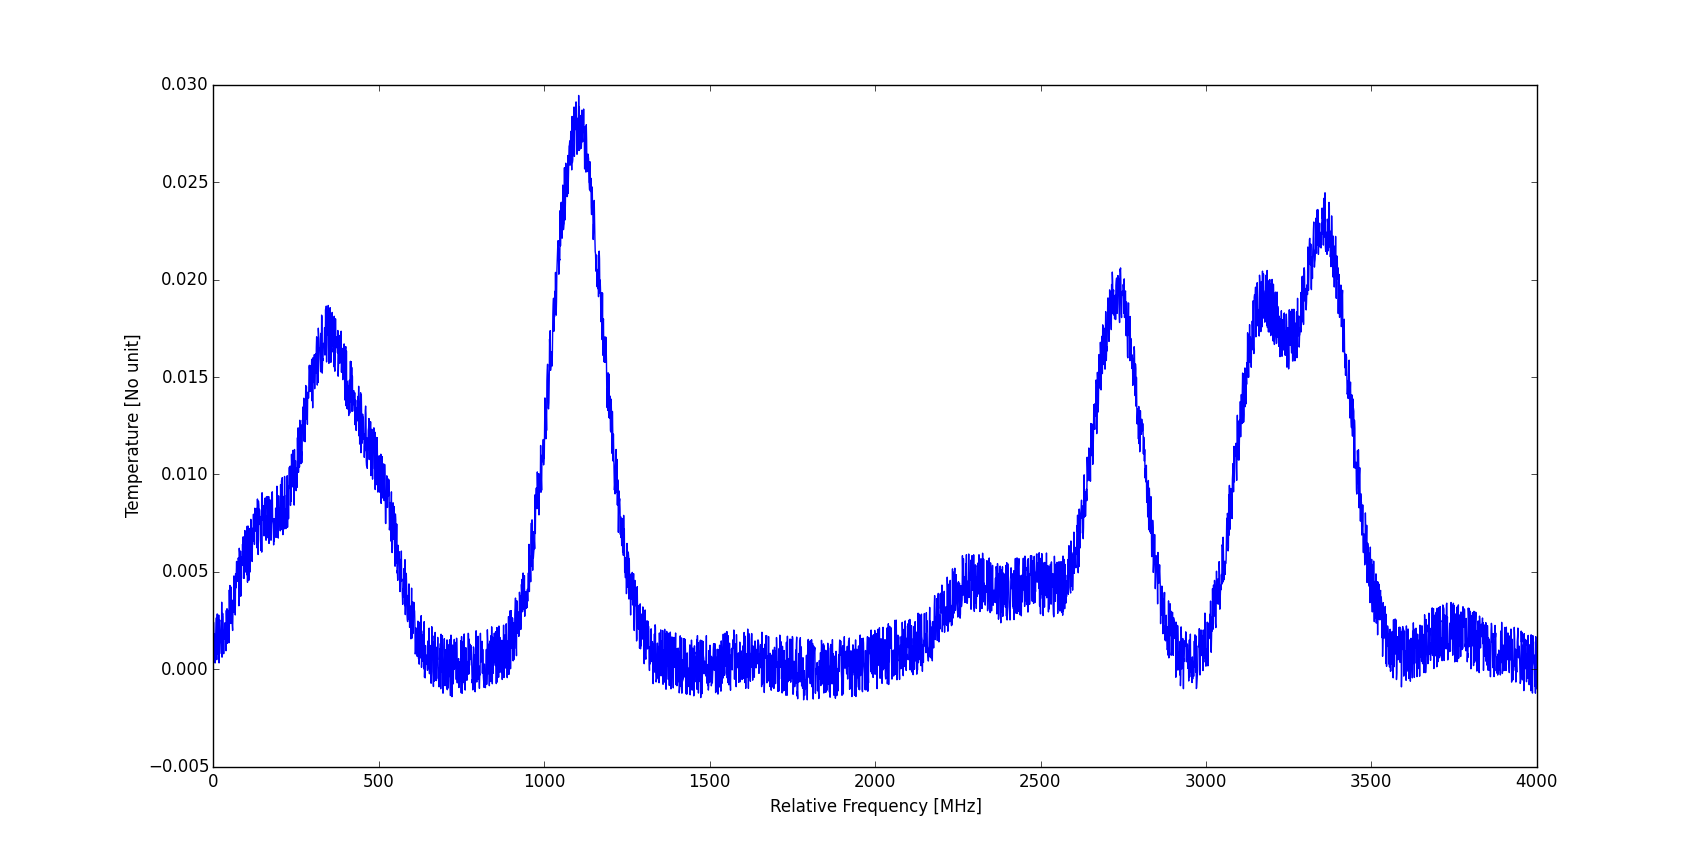
\includegraphics[width=140mm]{images/fig2}
		\caption{Espectro al situarse en un píxel espacial en particular. }
	\end{center}
\end{figure}

A continuación, para cada punto espacial del cubo de datos, se toma cada espectrograma de manera independiente. Lo primero es reducir el ruido de el espectro utilizando un filtro de Savitzky-Golay \cite{howley_effect_2005}. Este filtro utiliza un parámetro que indica el número de mediciones consecutivas a utilizar para suavizar la curva, por lo que el ancho de las curvas simuladas corresponde aun buen parámetro para ser asignado. Con este filtro se puede obtener un espectro con menor variación y así, identificar con mayor claridad las líneas. Este filtro se aplica al cubo completo, incluido el píxel con solo ruido, para hacer comparables los espectros al calcular la sensibilidad.

\begin{figure}[H]
	\begin{center}
		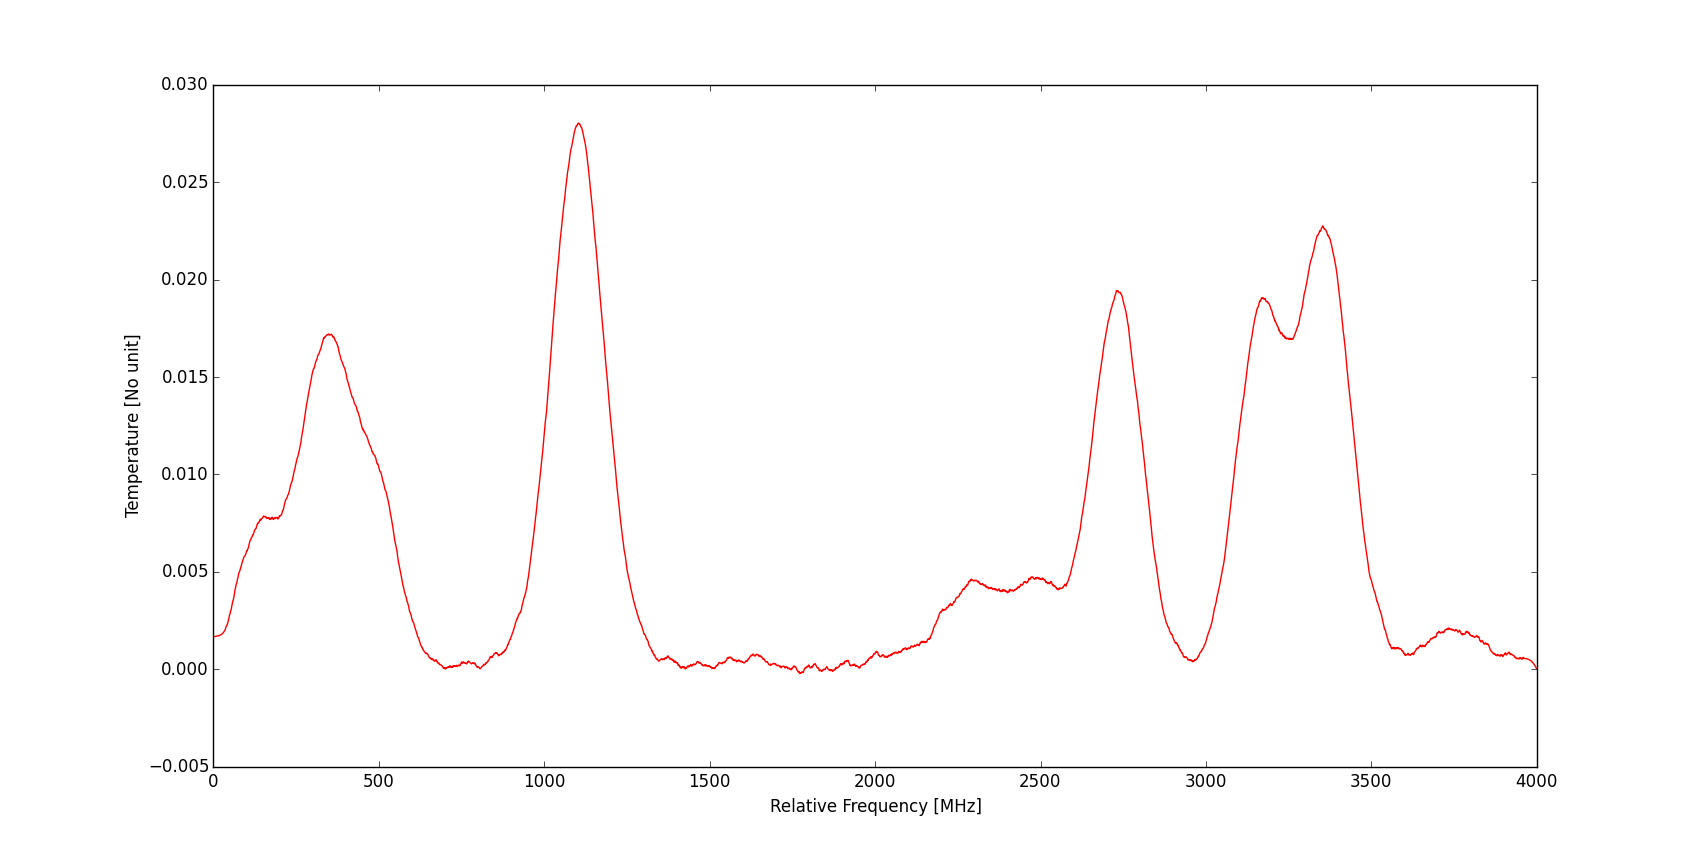
\includegraphics[width=140mm]{images/fig3}
		\caption{Espectro al reducir el ruido con un filtro de Savitzky-Golay. }
	\end{center}
\end{figure}


Se comienza con la determinación de los puntos máximos de la curva observada. Es posible asignar un parámetro que determina la distancia máxima que debe existir entre el brillo de dos frecuencias consecutivas para ser considerados un máximo. Sin este parámetro, la curva tendría una serie de falsos máximos y mínimos producto del ruido existente en las mediciones. Así, cada máximo local detectado que está por sobre el parámetro de sensibilidad es un candidato a línea de emisión.

\begin{figure}[H]
	\begin{center}
		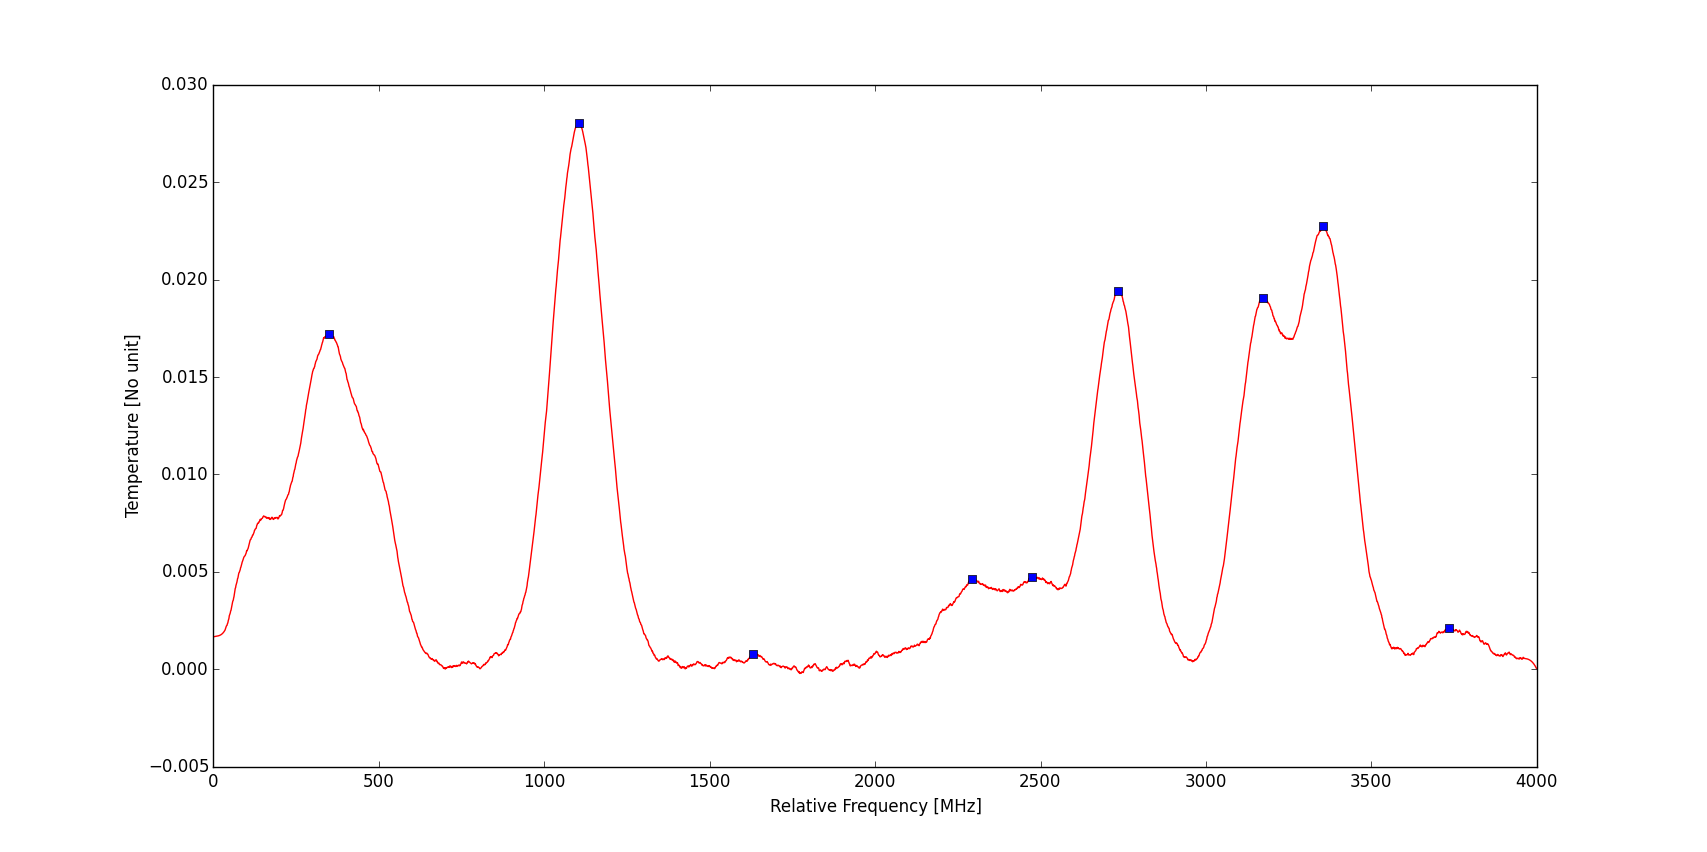
\includegraphics[width=140mm]{images/fig4}
		\caption{Puntos máximos locales por sobre el parámetro de sensibilidad. }
	\end{center}
\end{figure}

Al final del proceso, se crea un vector del tamaño del ancho de banda observado, donde se cada elemento del vector representa 1 Mhz del espectro. En cada frecuencia donde se detectó una línea, se asigna el valor 1, y cero en caso contrario.

\begin{figure}[H]
	\begin{center}
		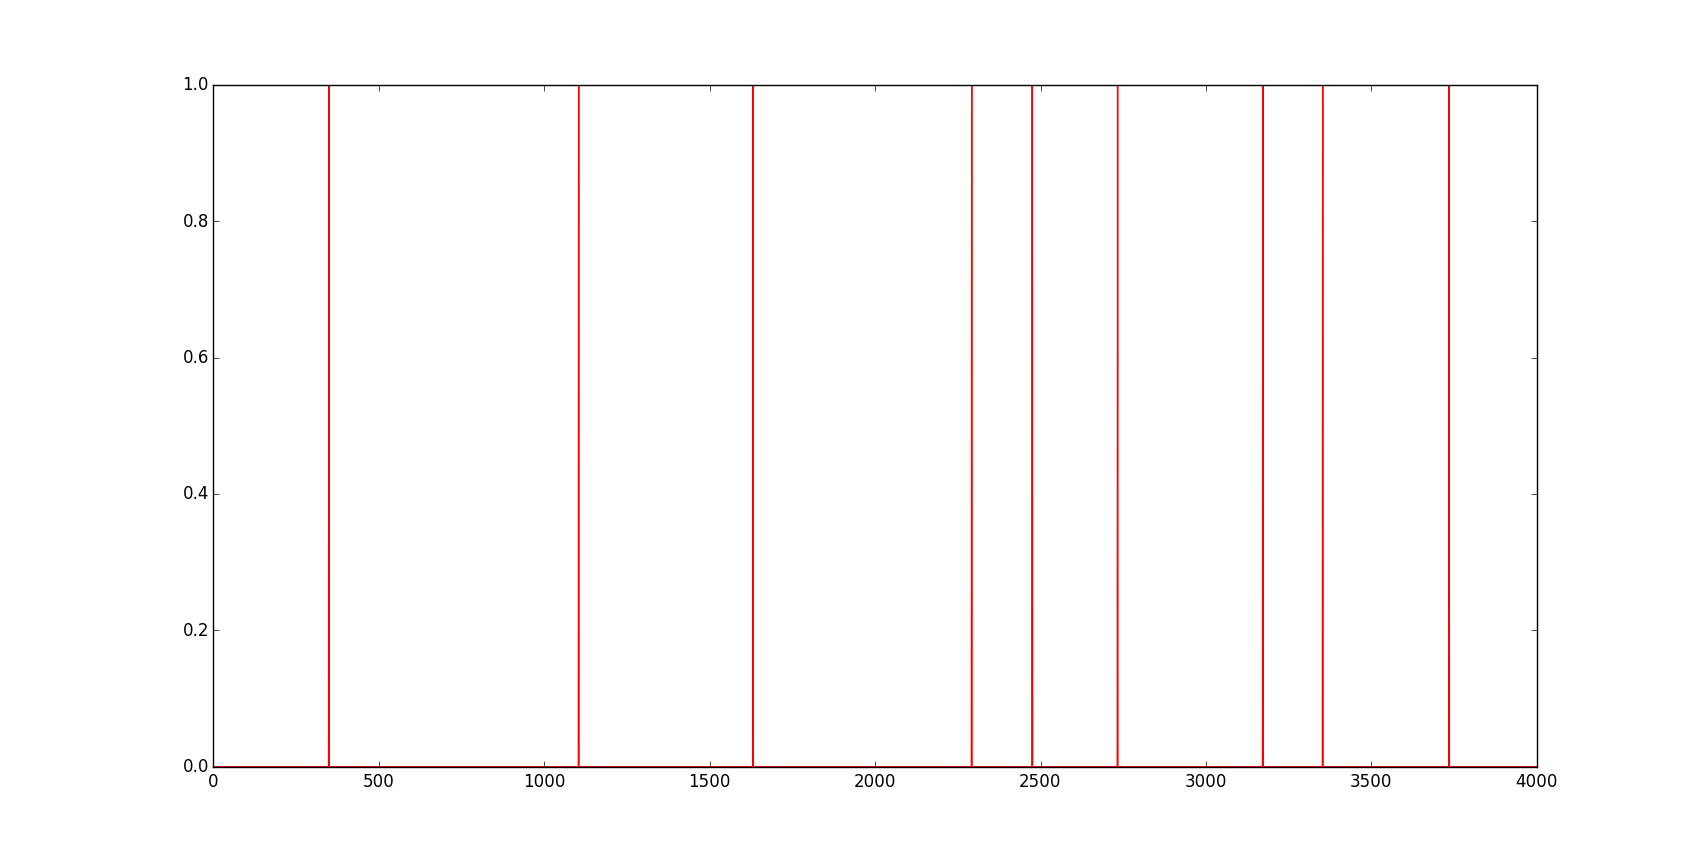
\includegraphics[width=140mm]{images/fig5}
		\caption{Gráfico del vector observado con valores no nulos en los puntos detectados. }
	\end{center}
\end{figure}

\begin {table}[H]
\begin{center}
	\begin{tabular}{|c|c|c|c|c|c|c|c|c|c|c|}
		\hline 0 & 0 &  ... &  1 & ... &  1 & ... & 1 & ... & 0 & 0 \\ 
		\hline
	\end{tabular}
	\caption {Forma del vector del espectro observado para el caso analizado.}
\end{center}
\end{table}

\subsubsection{Etapa de Predicción}

A continuación, se utiliza el catalogo de líneas espectroscópicas teóricas Splatalogue para obtener la lista de todas las frecuencias teóricas en el rango observado.

Para cada isotopo con líneas teóricas, se crea un vector del tamaño de la ventana en Mhz, similar al de la etapa de detección, donde el valor de cada posición es 1 si existe una línea teórica en dicha frecuencia para dicho isotopo, y cero en otro caso. Cada uno de estos vectores corresponde a una palabra de un diccionario de moléculas.

Posteriormente, se procesan las palabras de modo que solo tengan valores distintos de cero en las frecuencias donde el espectro observado es distinto de cero. Para esto, se asigna en dichas frecuencias la diferencia entre 1 y distancia exponencial entre la frecuencia observada y la frecuencia teórica más cercana, utilizando como parámetro sigma igual al ancho de las líneas espectrales.

Con esto se espera que las palabras que tienen frecuencias teóricas más cercanas a las observadas, tendrán valores mayores, con lo que el algoritmo de sparse coding tenga preferencia a elegir dichas palabras.

\begin{figure*}[ht]
	\centering
	\subfigure[Figura 6.1.]{
		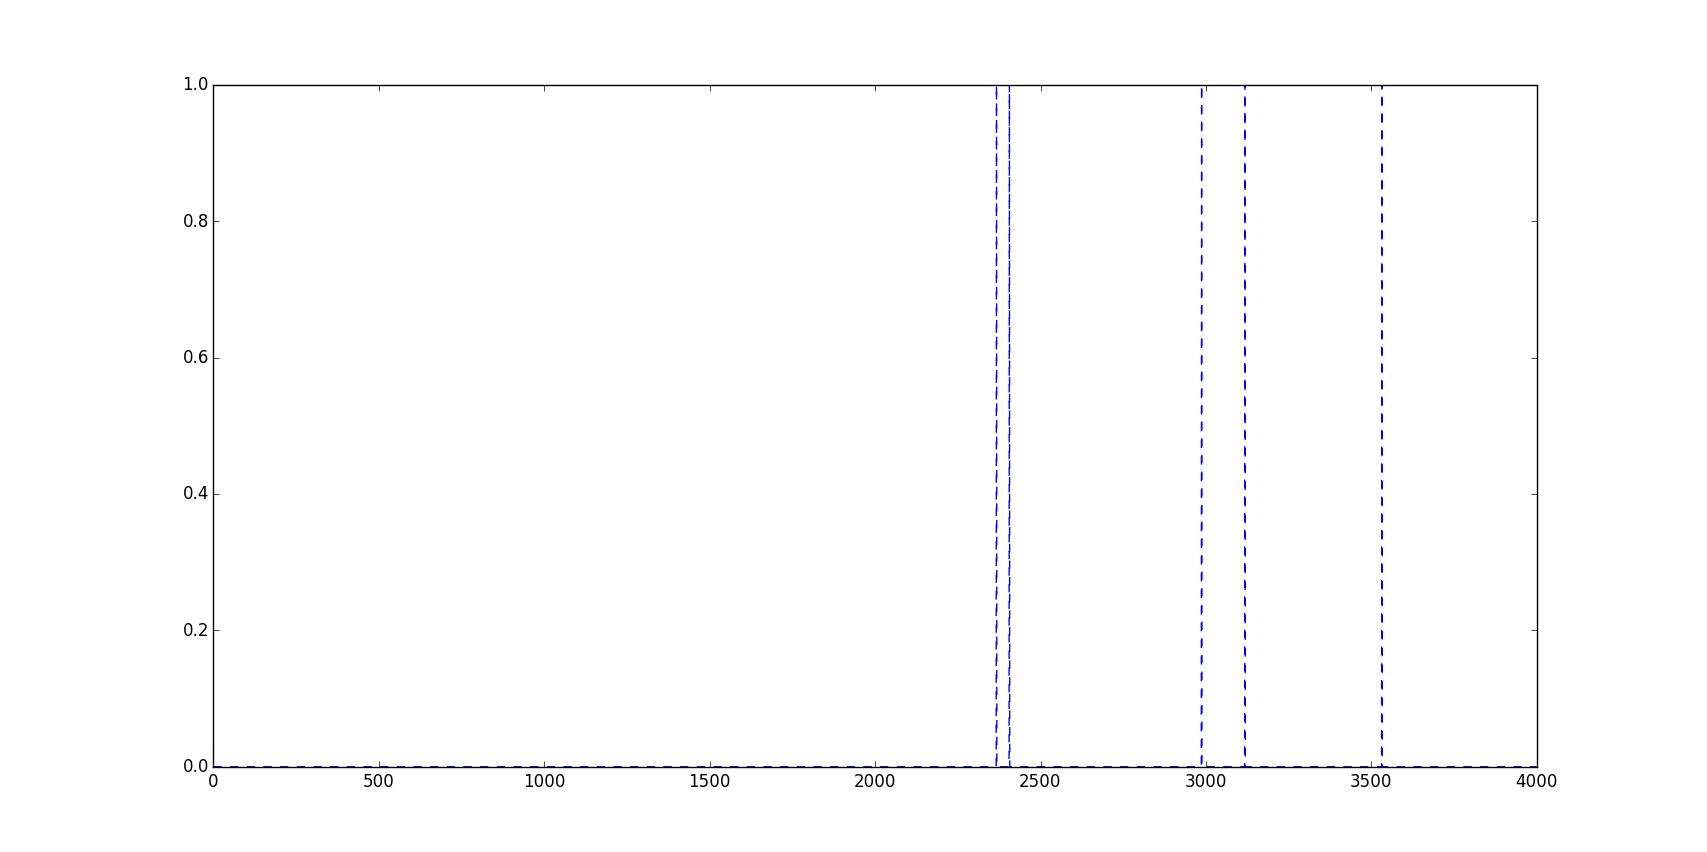
\includegraphics[width=100mm]{images/fig6-1}
	\label{subfig:fig6-1}
	}
	\subfigure[Figura 6.2.]{
		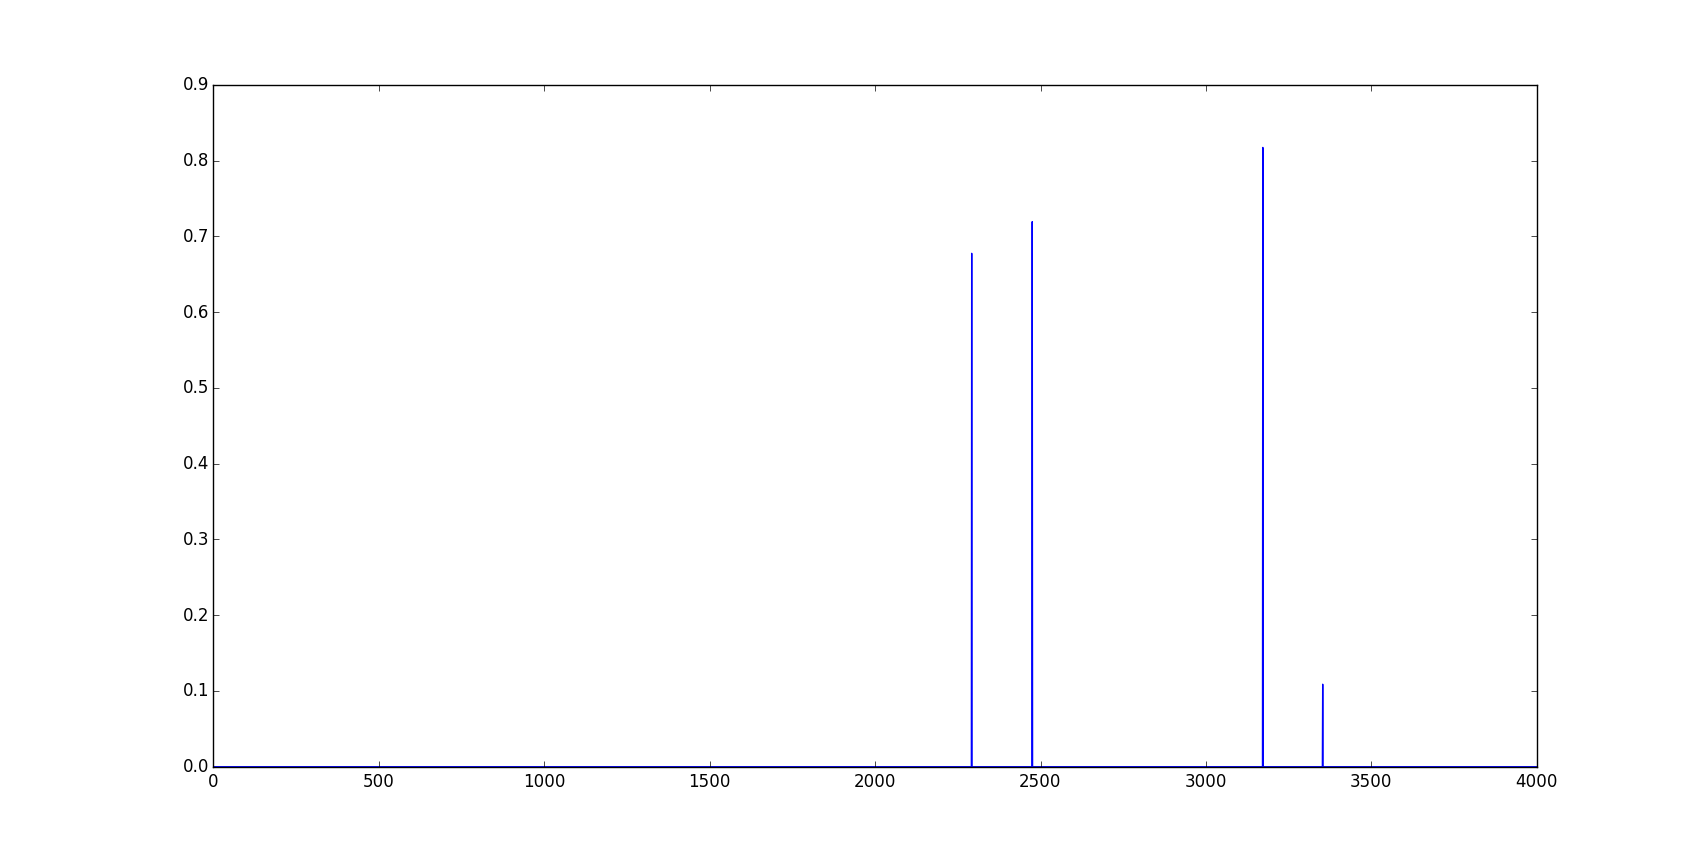
\includegraphics[width=100mm]{images/fig6-2}
		\label{subfig:fig6-2}
	}
	\caption{Rn la figura \ref{subfig:fig6-1} se grafica una palabra teórica y en la \ref{subfig:fig6-2} su equivalente recalculado}
\end{figure*}

La implementación se asegura de que cada frecuencia teórica cambie el valor de una y solo una frecuencia observada, y en caso de que haya otra frecuencia teórica que también tenga como frecuencia observada más cercana a la misma frecuencia, se asigna la menor distancia a dicha frecuencia observada. Con esto, cada palabra del diccionario queda con la misma o con menor cantidad de frecuencias distintas de cero.

\begin {table}[H]
\begin{center}
	\begin{tabular}{|c|c|c|c|c|c|c|c|c|c|c|c|}
		\hline Vector Obervado     & 0 & 0 &  0 &  1    & 0 &  1 & 0 & 1   & 0 & 0 & 0 \\ 
		\hline Palabra Teórica     & 0 & 0 &  1 &  0    & 0 &  1 & 0 & 0   & 0 & 0 & 1 \\ 
		\hline Palabra Recalculada & 0 & 0 &  0 &  0.88 & 0 &  1 & 0 & 0.6 & 0 & 0 & 0 \\ 
		\hline
	\end{tabular}
	\caption {Ejemplo de recálculo de una palabra utilizando para la distancia exponencial sigma = 2.}
\end{center}
\end{table}

Finalmente, se tiene un problema de optimización con una formulación de sparse coding, donde se intenta acercar  al máximo la combinación lineal entre palabras de tal forma que se construya el vector del espectro observado. El paramero de sparsity permite restringir la cantidad de palabras que se desea que el modelo utilice para formar la observación. En este caso se asignó un valor elevado para que el modelo pudiese acercarse lo máximo posible a la observación sin límite de palabras.  La función a minimizar en esta formulación es la norma l-2 y corresponde al error cuadrático medio.


\begin{center}
$min_{\alpha} ||x-D\alpha||_2^2$ 
$s.a.$ 
$||\alpha||_1 \leq \lambda$ \\
$x$ : vector observado, 
$D$ : diccionario recalculado, 
$\lambda$ : parámetro de spartity, 
$||()||_2$ : Norma l-2
\end{center}


La solución óptima debería utilizar solo las palabras asociadas a los isotopos presentes en el espectro. En la siguiente tabla se puede ver la simulación realizada y los isotopos rescatados:

\begin {table}[H]
\begin{center}
	\begin{tabular}{|c|c|c|}
		\hline Nombre & Fórmula &  Isótopos \\ 
		

		\hline	Hydrogen Cyanide & 'HCN' & 'HC15Nv=0', 'H13CNv2=1', 'H13CNv=0'\\ 
		
		\hline	Thioformaldehyde & 'H2CS' & 'H213CS' \\
		
		\hline	Sulfur Dioxide & 'SO2' & 'SO2v=0', 'SO2v2=1' \\
		
		\hline	Sulfur Dioxide & 'OSO' & 'OS18O', 'OS17O' \\
		
		\hline	Formaldehyde & 'H2CO'  & 'H2C18O', 'H213CO' \\
				
		\hline 
	\end{tabular}
	\caption {Conjunto de isótopos con los que se realizaron simuló la implementación.}
\end{center}
\end{table}

\begin {table}[H]
\begin{center}
	\begin{tabular}{|c|c|c|c|}
		\hline Nombre & Fórmula &  Isótopos & Alpha \\ 
		
		
		\hline	Hydrogen Cyanide & 'HCN'  & 'HC15Nv=0' & 0.0000\\
								 &		  & 'H13CNv2=1' & 0.0000\\
								 &		  & 'H13CNv=0' & 0.0000\\ 
								
		
		\hline	Thioformaldehyde & 'H2CS' & 'H213CS' & 0.0000\\
		
		\hline	Sulfur Dioxide & 'SO2'	  & 'SO2v=0' & 0.0000\\
								&		  & 'SO2v2=1'& 0.2694 \\
		
		\hline	Sulfur Dioxide & 'OSO' & 'OS18O' & 0.9612\\
							   &	   & 'OS17O' & 0.5589\\
		
		\hline	Formaldehyde & 'H2CO'  & 'H2C18O' & 0.0000\\
							 &		   & 'H213CO' & 0.0000\\
		
		\hline 
	\end{tabular}
	\caption {Conjunto de isótopos utilizados para la simulación y su valor de alpha.}
\end{center}
\end{table}

Cabe destacar que en este caso solo hubo un falso positivo, el isotopo '33SO2', con un valor de alpha de 0.6592. Esto significa que el algoritmo tiende a elegir los isotopos de moléculas con mayor cantidad de líneas en el ancho de banda observado, y es un aspecto a mejorar. 

Además, ciertas moléculas no son detectadas, y esto se puede deber a dos factores: en primer lugar, el algoritmo no logró detectarlas en la etapa anterior al no ser suficiente el filtro de ruido aplicado para que fuera identificada como máximo local o, en segundo lugar, no superó la sensibilidad dado que la variabilidad de la simulación hizo que no fuera observable. 

%\begin{figure}[H]
%	\begin{center}
%		
\includegraphics{images/fig1}
%		\caption{Espectro residual al sustraer una gausiana ajustada en una potencial línea de emisión. }
%	\end{center}
%\end{figure}

% Una forma de validación del algoritmo consiste en tomar un solo punto espacial del cubo como entrenamiento del algoritmo, y el resto de los pixeles como test de validación. De esta forma las palabras teóricas se recalcularán según las observaciones de dicho píxel espacial. En el resto de los píxeles del cubo, la variabilidad producto del effecto doppler interno y propia de la simulación  debería generar variaciones de forma que ciertas líneas se manifestarían y ciertas dejarían de observarse, a pesar de tener la misma composición.

% Si el algoritmo puede predecir los compuestos detectados en el píxel de referencia en el resto del cubo, se validaría esta aproximación al problema. De esta forma, se procedió a evaluar el algoritmo, obteniendo los siguientes resultados:



